\documentclass[12pt,a4paper]{article}

\usepackage[utf8]{inputenc}
\usepackage[T2A]{fontenc}
\usepackage[russian]{babel}
\usepackage{amsmath}
\usepackage{amssymb}
\usepackage{array}
\usepackage{booktabs}
\usepackage{caption}
\usepackage{enumitem}
\usepackage{fancyhdr}
\usepackage{float}
\usepackage{geometry}
\usepackage{graphicx}
\usepackage{hyperref}
\usepackage{indentfirst}
\usepackage{listings}
\usepackage{longtable}
\usepackage{tikz}
\usepackage{xcolor}
\usetikzlibrary{arrows.meta,positioning,shapes.geometric}

\geometry{left=30mm,right=15mm,top=20mm,bottom=20mm}
\setlength{\parindent}{1.25cm}
\linespread{1.2}
\pagestyle{fancy}
\fancyhf{}
\fancyfoot[C]{\thepage}
\renewcommand{\headrulewidth}{0pt}
\hypersetup{hidelinks}

\captionsetup{justification=centering}
\setcounter{tocdepth}{2}

\definecolor{codebg}{RGB}{248,248,248}
\definecolor{codeframe}{RGB}{215,215,215}
\definecolor{codekw}{RGB}{0,76,153}
\definecolor{codestr}{RGB}{163,21,21}
\definecolor{codecomment}{RGB}{0,128,0}

\lstdefinelanguage{JavaScript}{
  morekeywords={const,let,var,function,return,if,else,for,while,throw,new,export,import,from,class,get},
  sensitive=true,
  morecomment=[l]{//},
  morestring=[b]",
  morestring=[b]',
}

\lstset{
  language=JavaScript,
  basicstyle=\ttfamily\small,
  keywordstyle=\color{codekw}\bfseries,
  stringstyle=\color{codestr},
  commentstyle=\color{codecomment},
  backgroundcolor=\color{codebg},
  frame=single,
  rulecolor=\color{codeframe},
  numbers=left,
  numberstyle=\tiny,
  stepnumber=1,
  breaklines=true,
  showstringspaces=false,
  tabsize=2,
  columns=fullflexible,
  keepspaces=true,
  extendedchars=true,
  inputencoding=utf8
}

\newcolumntype{C}[1]{>{\centering\arraybackslash}p{#1}}

\begin{document}

% ====================== ТИТУЛЬНЫЙ ЛИСТ ======================
\pagenumbering{gobble}
\hypersetup{pageanchor=false}
\begin{titlepage}
  \thispagestyle{empty}
  \begin{center}
    {\small Федеральное государственное автономное образовательное учреждение высшего образования\\
    «Национальный исследовательский университет ИТМО»}\\[0.8em]
    {\small Факультет программной инженерии и компьютерной техники}

    \vfill

    {\Large\textbf{Лабораторная работа №4}}\\[0.6em]
    {\large по курсу «Вычислительная математика»}\\[0.6em]
    {\large Вариант 19}

    \vfill

    \begin{flushright}
      \begin{tabular}{l}
        Выполнил:\\
        Якименко Владислав Игоревич, Р3213\\[0.8em]
        Проверила:\\
        Малышева Татьяна Алексеевна
      \end{tabular}
    \end{flushright}

    \vfill

    Санкт-Петербург --- 2026
  \end{center}
\end{titlepage}
\clearpage
\hypersetup{pageanchor=true}

\tableofcontents
\thispagestyle{empty}
\clearpage
\pagenumbering{arabic}

% ====================== РАЗДЕЛ 1 ======================
\section{Вычислительная реализация задачи}

\subsection{Постановка задачи}

\textbf{Задание:}
\begin{enumerate}[label=\arabic*., leftmargin=1.2cm]
  \item Сформировать таблицу табулирования заданной функции на указанном интервале.
  \item Построить линейное и квадратичное приближения по 11 точкам заданного интервала.
  \item Найти среднеквадратические отклонения для каждой аппроксимирующей функции.
  \item Выбрать наилучшее приближение.
  \item Построить графики заданной функции, а также полученных линейного и квадратичного приближений.
  \item Привести подробные вычисления.
\end{enumerate}

\textbf{Функция вычислительной части (вариант 19):}
\[
  y=f(x)=\frac{5x}{x^4+19},\qquad x\in[0;\,2],\qquad h=0.2.
\]

\subsection{Графическое представление}

Построим график исходной функции $f(x)$, линейного приближения $\varphi_1(x)$
и квадратичного приближения $\varphi_2(x)$ на исследуемом интервале.

\begin{figure}[H]
  \centering
  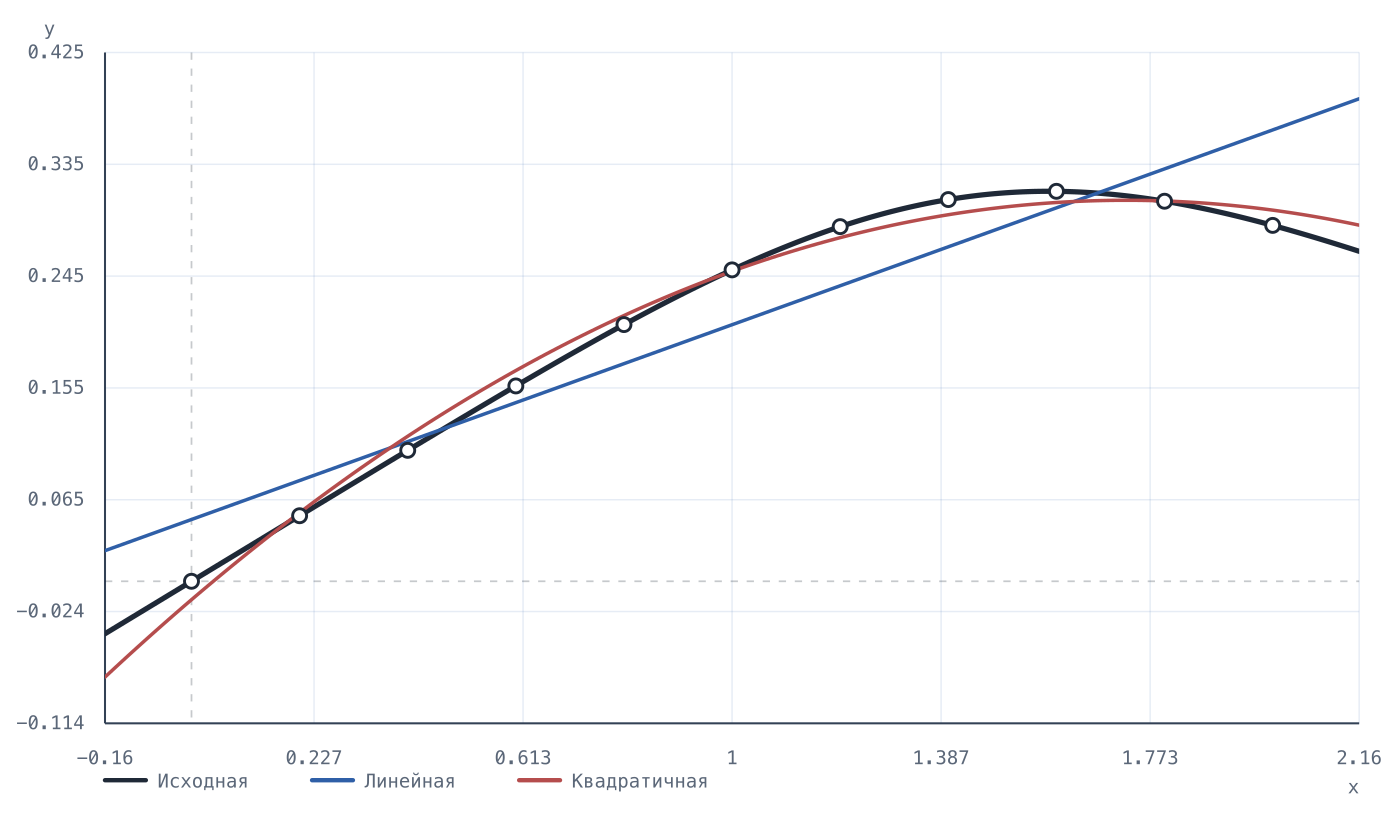
\includegraphics[width=0.96\textwidth]{docs/graph-computational.png}
  \caption{Исходная функция и аппроксимирующие функции на отрезке $[0;\,2]$}
\end{figure}

По графику видно, что линейная функция описывает только общий рост табличных значений,
а квадратичная функция лучше учитывает максимум функции на правой части интервала.

\subsection{Рабочие формулы метода}

Мерой отклонения аппроксимирующей функции $\varphi(x)$ от табличной функции является
сумма квадратов отклонений:
\[
  S=\sum_{i=1}^{n}\left(\varphi(x_i)-y_i\right)^2\rightarrow\min.
\]

Среднеквадратическое отклонение:
\[
  \delta=\sqrt{\frac{S}{n}}.
\]

Для полинома степени $m$
\[
  \varphi(x)=a_0+a_1x+a_2x^2+\dots+a_mx^m
\]
коэффициенты находятся из нормальной системы:
\[
  \sum_{j=0}^{m}a_j\sum_{i=1}^{n}x_i^{j+k}=
  \sum_{i=1}^{n}x_i^k y_i,\qquad k=0,1,\dots,m.
\]

Для линейной зависимости дополнительно вычисляется коэффициент корреляции Пирсона:
\[
  r=\frac{\sum_{i=1}^{n}(x_i-\bar{x})(y_i-\bar{y})}
  {\sqrt{\sum_{i=1}^{n}(x_i-\bar{x})^2\sum_{i=1}^{n}(y_i-\bar{y})^2}}.
\]

Коэффициент детерминации:
\[
  R^2=1-\frac{\sum_{i=1}^{n}(y_i-\varphi(x_i))^2}
  {\sum_{i=1}^{n}(y_i-\bar{y})^2}.
\]

\begin{figure}[H]
  \centering
  \begin{tikzpicture}[
    node distance=0.75cm,
    >=Stealth,
    flowline/.style={->, line width=0.45pt, draw=black!70},
    block/.style={
      draw=black!55,
      line width=0.6pt,
      align=center,
      minimum width=9.2cm,
      minimum height=0.95cm,
      inner sep=4pt
    },
    io/.style={
      block,
      trapezium,
      trapezium left angle=70,
      trapezium right angle=110
    },
    process/.style={block, rectangle},
    loop/.style={
      draw=black!55,
      line width=0.6pt,
      align=center,
      regular polygon,
      regular polygon sides=6,
      shape border rotate=30,
      minimum width=4.3cm,
      minimum height=0.72cm,
      inner sep=1pt
    }
  ]
    \node[io] (input) {Ввод исходных значений:\\ $(x_i)$, $(y_i)$, $n$};
    \node[process, below=of input] (sums) {
      $\displaystyle \sum_{i=1}^{n}x_i,\quad
      \sum_{i=1}^{n}x_i^2,\quad
      \sum_{i=1}^{n}y_i,\quad
      \sum_{i=1}^{n}x_iy_i$
    };
    \node[process, below=of sums] (system) {
      Решение системы линейных уравнений:\\ вычисление $a$, $b$
    };
    \node[loop, below=of system] (cycle) {$i=1,\ldots,n$};
    \node[process, below=of cycle] (values) {
      $\hat{y}_i=ax_i+b,\qquad
      \varepsilon_i=\hat{y}_i-y_i,\qquad
      p_i=\dfrac{\varepsilon_i}{y_i}$
    };
    \node[process, below=of values] (stats) {
      $\displaystyle S=\sum_{i=1}^{n}\varepsilon_i^2,\qquad r$
    };
    \node[io, below=of stats] (output) {
      Вывод результатов:\\ $x_i$, $y_i$, $\hat{y}_i$, $\varepsilon_i$, $p_i$, $a$, $b$, $S$, $r$
    };

    \draw[flowline] (input) -- (sums);
    \draw[flowline] (sums) -- (system);
    \draw[flowline] (system) -- (cycle);
    \draw[flowline] (cycle) -- (values);
    \draw[flowline] (values) -- (stats);
    \draw[flowline] (stats) -- (output);
    \draw[flowline] (stats.west) -- ++(-1.1,0) |- (cycle.west);
  \end{tikzpicture}
  \caption{Блок-схема алгоритма линейной аппроксимации методом наименьших квадратов}
\end{figure}

\subsection{Таблица табулирования функции}

\begin{table}[H]
  \centering
  \caption{Точки табулирования функции $f(x)=\dfrac{5x}{x^4+19}$}
  \begin{tabular}{C{1cm}C{1.7cm}C{2.4cm}C{1cm}C{1.7cm}C{2.4cm}}
    \toprule
    $i$ & $x_i$ & $y_i$ & $i$ & $x_i$ & $y_i$ \\
    \midrule
    1 & 0.0 & 0.000000 & 7 & 1.2 & 0.284716 \\
    2 & 0.2 & 0.052627 & 8 & 1.4 & 0.306458 \\
    3 & 0.4 & 0.105122 & 9 & 1.6 & 0.313067 \\
    4 & 0.6 & 0.156825 & 10 & 1.8 & 0.305110 \\
    5 & 0.8 & 0.206084 & 11 & 2.0 & 0.285714 \\
    6 & 1.0 & 0.250000 & & & \\
    \bottomrule
  \end{tabular}
\end{table}

Вычисленные суммы для нормальных уравнений:

\begin{table}[H]
  \centering
  \caption{Суммы для метода наименьших квадратов}
  \begin{tabular}{C{3.3cm}C{3.2cm}C{3.3cm}C{3.2cm}}
    \toprule
    \textbf{Величина} & \textbf{Значение} & \textbf{Величина} & \textbf{Значение} \\
    \midrule
    $n$ & 11 & $\sum y_i$ & 2.265723 \\
    $\sum x_i$ & 11.000000 & $\sum x_iy_i$ & 2.953771 \\
    $\sum x_i^2$ & 15.400000 & $\sum x_i^2y_i$ & 4.400790 \\
    $\sum x_i^3$ & 24.200000 & $\sum x_i^3y_i$ & 7.076887 \\
    $\sum x_i^4$ & 40.532800 & $\sum x_i^5$ & 70.664000 \\
    $\sum x_i^6$ & 126.617920 & & \\
    \bottomrule
  \end{tabular}
\end{table}

\subsection{Линейное приближение}

Ищем функцию вида
\[
  \varphi_1(x)=a_1x+a_0.
\]

Нормальная система:
\[
\begin{cases}
  11a_0+11a_1=2.265723,\\
  11a_0+15.4a_1=2.953771.
\end{cases}
\]

Решение системы:
\[
  a_0=0.049600,\qquad a_1=0.156374.
\]

Итак,
\[
  \boxed{\varphi_1(x)=0.156374x+0.049600}.
\]

\begin{table}[H]
  \centering
  \caption{Значения линейного приближения}
  \begin{tabular}{C{0.8cm}C{1.4cm}C{2.2cm}C{2.4cm}C{2.2cm}}
    \toprule
    $i$ & $x_i$ & $y_i$ & $\varphi_1(x_i)$ & $\varepsilon_i$ \\
    \midrule
    1 & 0.0 & 0.000000 & 0.049600 & 0.049600 \\
    2 & 0.2 & 0.052627 & 0.080875 & 0.028248 \\
    3 & 0.4 & 0.105122 & 0.112150 & 0.007029 \\
    4 & 0.6 & 0.156825 & 0.143425 & -0.013400 \\
    5 & 0.8 & 0.206084 & 0.174700 & -0.031384 \\
    6 & 1.0 & 0.250000 & 0.205975 & -0.044025 \\
    7 & 1.2 & 0.284716 & 0.237250 & -0.047467 \\
    8 & 1.4 & 0.306458 & 0.268525 & -0.037934 \\
    9 & 1.6 & 0.313067 & 0.299800 & -0.013268 \\
    10 & 1.8 & 0.305110 & 0.331074 & 0.025965 \\
    11 & 2.0 & 0.285714 & 0.362349 & 0.076635 \\
    \bottomrule
  \end{tabular}
\end{table}

\[
  S_1=0.016825,\qquad \delta_1=\sqrt{\frac{0.016825}{11}}=\boxed{0.039}.
\]

Коэффициент корреляции Пирсона для линейной зависимости:
\[
  r=0.929929.
\]

\subsection{Квадратичное приближение}

Ищем функцию вида
\[
  \varphi_2(x)=a_2x^2+a_1x+a_0.
\]

Нормальная система:
\[
\begin{cases}
  11a_0+11a_1+15.4a_2=2.265723,\\
  11a_0+15.4a_1+24.2a_2=2.953771,\\
  15.4a_0+24.2a_1+40.5328a_2=4.400790.
\end{cases}
\]

Решение системы:
\[
  a_0=-0.014787,\qquad a_1=0.370999,\qquad a_2=-0.107312.
\]

Итак,
\[
  \boxed{\varphi_2(x)=-0.107312x^2+0.370999x-0.014787}.
\]

\begin{table}[H]
  \centering
  \caption{Значения квадратичного приближения}
  \begin{tabular}{C{0.8cm}C{1.4cm}C{2.2cm}C{2.4cm}C{2.2cm}}
    \toprule
    $i$ & $x_i$ & $y_i$ & $\varphi_2(x_i)$ & $\varepsilon_i$ \\
    \midrule
    1 & 0.0 & 0.000000 & -0.014787 & -0.014787 \\
    2 & 0.2 & 0.052627 & 0.055120 & 0.002493 \\
    3 & 0.4 & 0.105122 & 0.116443 & 0.011321 \\
    4 & 0.6 & 0.156825 & 0.169180 & 0.012355 \\
    5 & 0.8 & 0.206084 & 0.213332 & 0.007249 \\
    6 & 1.0 & 0.250000 & 0.248900 & -0.001100 \\
    7 & 1.2 & 0.284716 & 0.275882 & -0.008834 \\
    8 & 1.4 & 0.306458 & 0.294280 & -0.012179 \\
    9 & 1.6 & 0.313067 & 0.304092 & -0.008975 \\
    10 & 1.8 & 0.305110 & 0.305320 & 0.000210 \\
    11 & 2.0 & 0.285714 & 0.297962 & 0.012248 \\
    \bottomrule
  \end{tabular}
\end{table}

\[
  S_2=0.001016,\qquad \delta_2=\sqrt{\frac{0.001016}{11}}=\boxed{0.010}.
\]

\subsection{Сравнение результатов}

\begin{table}[H]
  \centering
  \caption{Сравнение линейного и квадратичного приближений}
  \begin{tabular}{C{5.5cm}C{3.2cm}C{3.2cm}}
    \toprule
    \textbf{Приближение} & \textbf{$S$} & \textbf{$\delta$} \\
    \midrule
    Линейное & 0.016825 & 0.039 \\
    Квадратичное & 0.001016 & 0.010 \\
    \bottomrule
  \end{tabular}
\end{table}

Наилучшим среди двух приближений является квадратичное, так как
$\delta_2<\delta_1$.

% ====================== РАЗДЕЛ 2 ======================
\section{Программная реализация}

Проект написан на JavaScript. Консольная часть запускается через Node.js, для визуализации
дополнительно сделан web-интерфейс в браузере. Программа принимает таблицу из 8--12 точек,
строит все требуемые аппроксимирующие функции, вычисляет меру отклонения $S$,
среднеквадратическое отклонение $\delta$, коэффициент детерминации $R^2$, коэффициент
корреляции Пирсона для линейной модели и выбирает лучшую функцию по минимальному
значению $\delta$.

\subsection{Листинг программы}

Построение нормальной системы для полиномиальной аппроксимации:

\begin{lstlisting}
export function leastSquaresPolynomial(points, degree) {
  const size = degree + 1;
  const matrix = Array.from({ length: size }, () => Array(size).fill(0));
  const vector = Array(size).fill(0);

  for (let row = 0; row < size; row += 1) {
    for (let column = 0; column < size; column += 1) {
      matrix[row][column] = sum(points.map((point) =>
        point.x ** (row + column)));
    }
    vector[row] = sum(points.map((point) =>
      point.y * point.x ** row));
  }

  return gaussianElimination(matrix, vector);
}
\end{lstlisting}

Расчёт статистик аппроксимации:

\begin{lstlisting}
function calculateStats(points, evaluate) {
  const values = points.map((point) => {
    const approximation = evaluate(point.x);
    const residual = approximation - point.y;
    return { x: point.x, y: point.y, approximation, residual };
  });

  const s = sum(values.map((row) => row.residual ** 2));
  const sigma = Math.sqrt(s / points.length);
  const yMean = mean(points.map((point) => point.y));
  const totalScatter = sum(points.map((point) =>
    (point.y - yMean) ** 2));
  const r2 = 1 - s / totalScatter;

  return { values, s, sigma, r2 };
}
\end{lstlisting}

Линеаризация неполиномиальных функций:

\begin{lstlisting}
function fitExponential(points) {
  requireDomain(points, (point) => point.y > 0);
  const transformed = points.map((point) =>
    ({ x: point.x, y: Math.log(point.y) }));
  const [lnA, b] = leastSquaresPolynomial(transformed, 1);
  const a = Math.exp(lnA);
  return createModel("exponential", points, { a, b },
    (x) => a * Math.exp(b * x));
}

function fitPower(points) {
  requireDomain(points, (point) => point.x > 0 && point.y > 0);
  const transformed = points.map((point) =>
    ({ x: Math.log(point.x), y: Math.log(point.y) }));
  const [lnA, b] = leastSquaresPolynomial(transformed, 1);
  const a = Math.exp(lnA);
  return createModel("power", points, { a, b }, (x) => a * x ** b);
}
\end{lstlisting}

\subsection{Результаты выполнения программы}

Для исходного набора варианта 19 программа получила следующие результаты:

\begin{table}[H]
  \centering
  \caption{Результаты программы для варианта 19}
  \begin{tabular}{C{4.7cm}C{2.4cm}C{2.4cm}C{2.8cm}}
    \toprule
    \textbf{Модель} & \textbf{$S$} & \textbf{$\delta$} & \textbf{$R^2$} \\
    \midrule
    Линейная & 0.01682546 & 0.03910993 & 0.86476730 \\
    Полиномиальная 2-й степени & 0.00101641 & 0.00961256 & 0.99183068 \\
    Полиномиальная 3-й степени & 0.00002656 & 0.00155375 & 0.99978656 \\
    Экспоненциальная & не применима & --- & --- \\
    Логарифмическая & не применима & --- & --- \\
    Степенная & не применима & --- & --- \\
    \bottomrule
  \end{tabular}
\end{table}

Экспоненциальная, логарифмическая и степенная модели неприменимы к исходной таблице
варианта 19, поскольку в ней есть точка $(0;\,0)$, а линеаризация этих моделей требует
положительных $x$ и/или $y$.

Лучшее применимое приближение:
\[
  \varphi(x)=-0.050036x^3+0.042797x^2+0.256515x-0.000376.
\]

Для положительного тестового набора, где применимы все шесть моделей, получены результаты:

\begin{table}[H]
  \centering
  \caption{Результаты программы для положительного тестового набора}
  \begin{tabular}{C{4.7cm}C{2.4cm}C{2.4cm}C{2.8cm}}
    \toprule
    \textbf{Модель} & \textbf{$S$} & \textbf{$\delta$} & \textbf{$R^2$} \\
    \midrule
    Линейная & 0.00047389 & 0.00725633 & 0.99984697 \\
    Полиномиальная 2-й степени & 0.00047385 & 0.00725605 & 0.99984698 \\
    Полиномиальная 3-й степени & 0.00042496 & 0.00687155 & 0.99986277 \\
    Экспоненциальная & 0.04569543 & 0.07125497 & 0.98524409 \\
    Логарифмическая & 0.09150904 & 0.10083487 & 0.97045003 \\
    Степенная & 0.01081343 & 0.03466255 & 0.99650814 \\
    \bottomrule
  \end{tabular}
\end{table}

Для некорректного набора из семи точек программа завершилась с диагностикой:
\[
  \texttt{Ошибка: Таблица должна содержать от 8 до 12 точек.}
\]

\subsection{Веб-интерфейс}

Для лабораторной работы реализован web-интерфейс, позволяющий редактировать таблицу точек,
загружать данные из файла, запускать расчёт, просматривать таблицу отклонений и график.
График можно масштабировать кнопками или колесом мыши, а также перемещать перетаскиванием.

\begin{figure}[H]
  \centering
  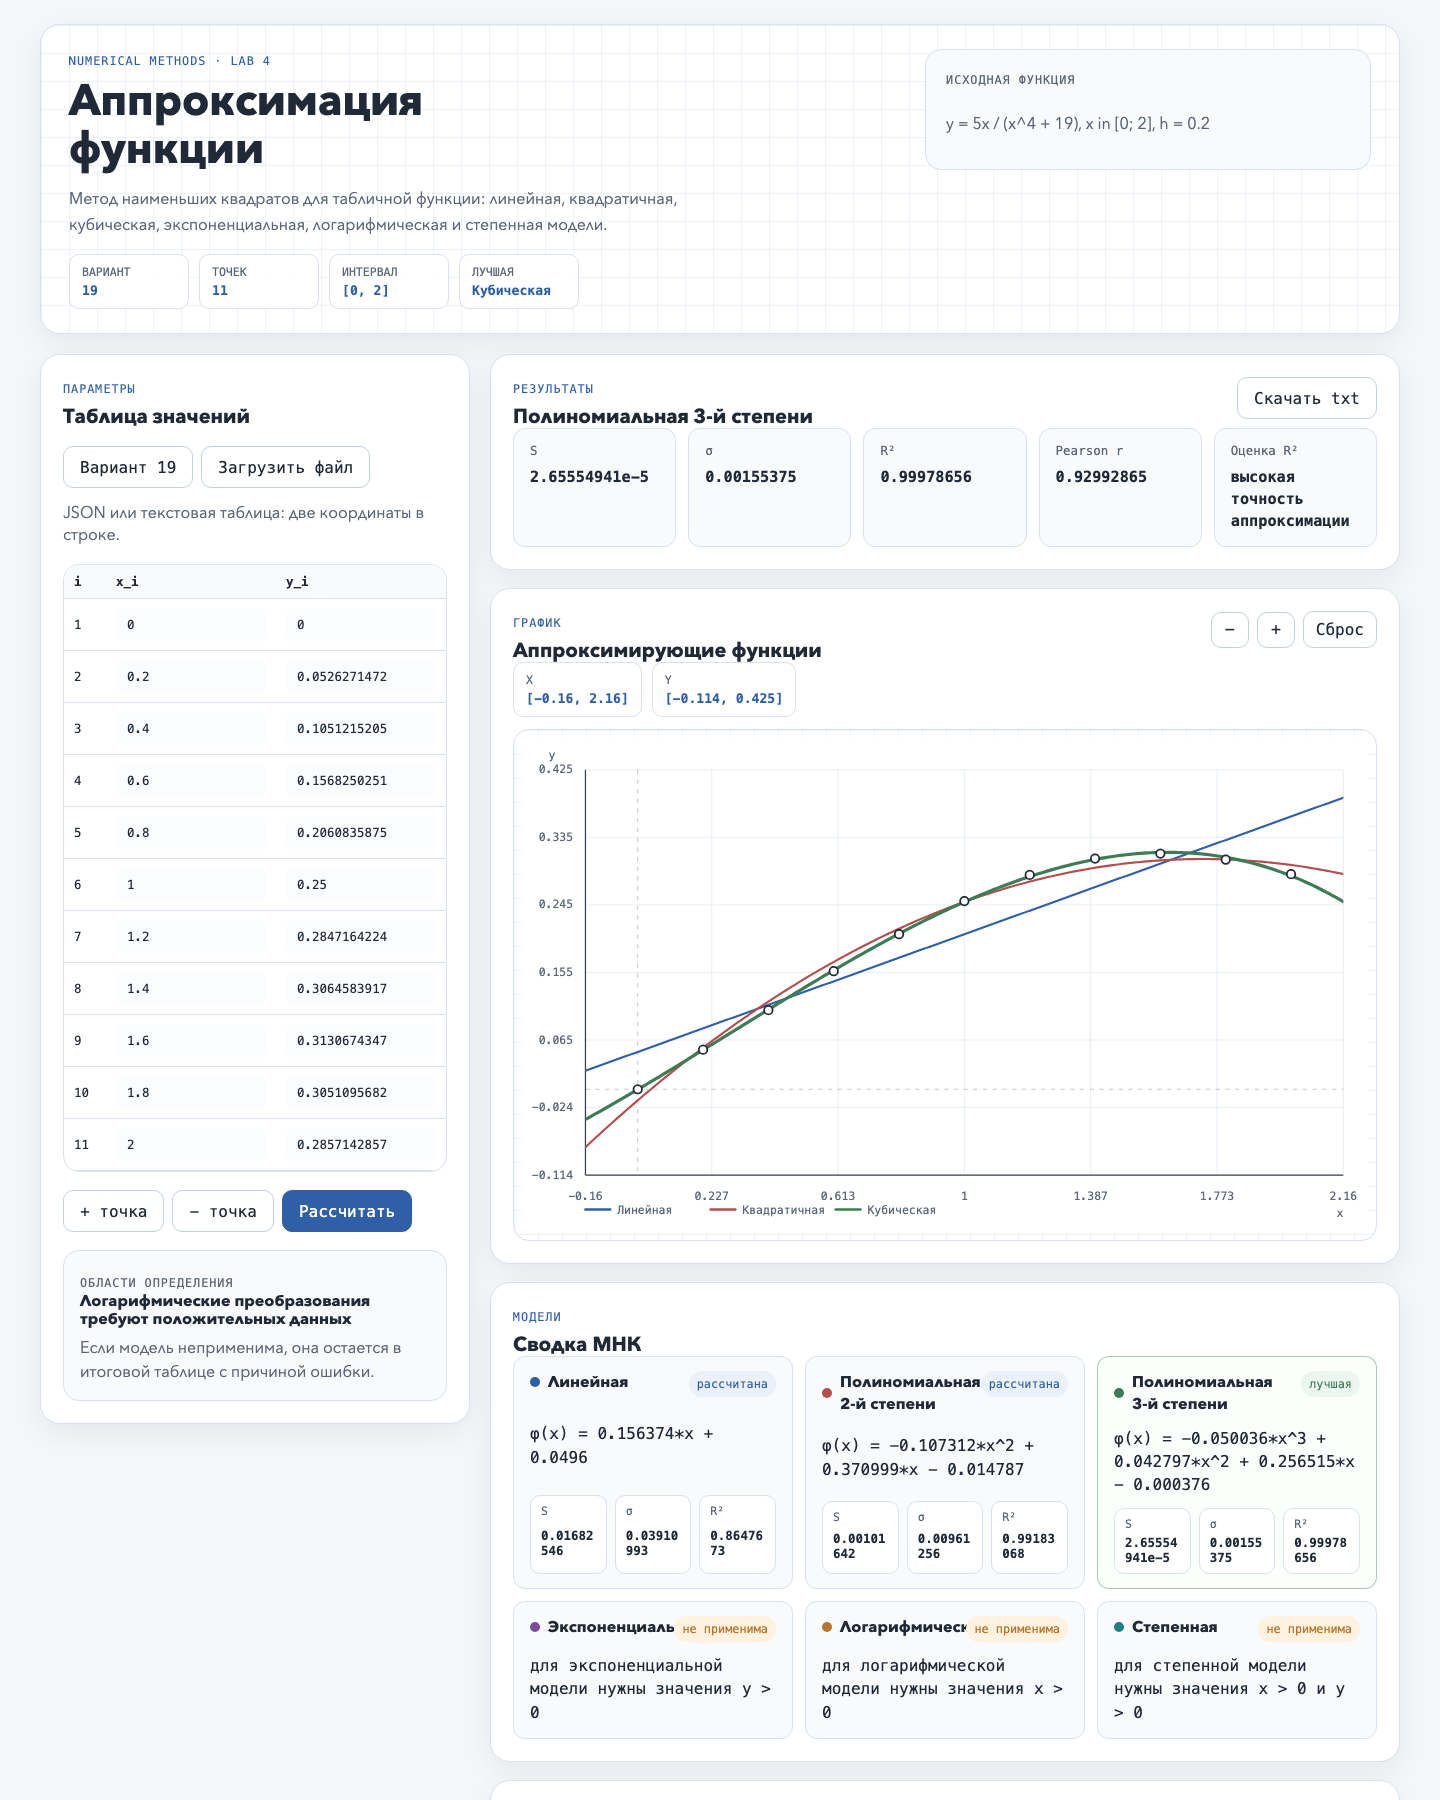
\includegraphics[width=\textwidth,height=0.86\textheight,keepaspectratio]{docs/screen-web-desktop.png}
  \caption{Веб-интерфейс: таблица исходных данных, метрики и интерактивный график}
\end{figure}

\begin{figure}[H]
  \centering
  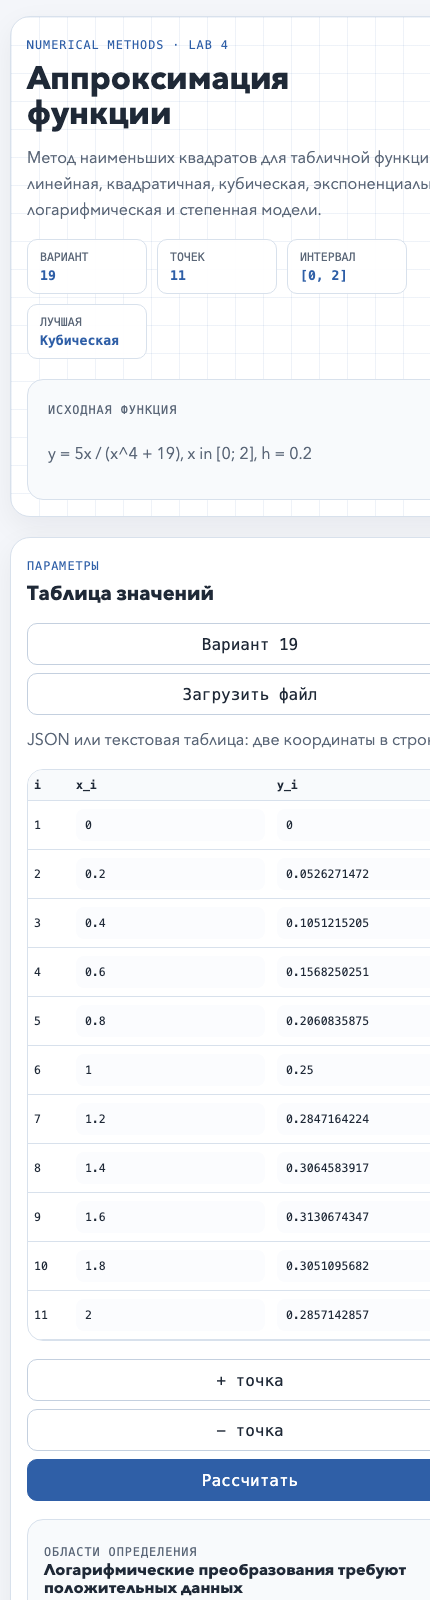
\includegraphics[width=0.62\textwidth,height=0.86\textheight,keepaspectratio]{docs/screen-web-mobile.png}
  \caption{Веб-интерфейс в узком окне: адаптивная форма ввода данных}
\end{figure}

\subsection{Проверка программы}

\begin{table}[H]
  \centering
  \caption{Наборы данных для проверки}
  \begin{tabular}{C{4cm}C{6.2cm}C{3.2cm}}
    \toprule
    \textbf{Набор} & \textbf{Содержание проверки} & \textbf{Результат} \\
    \midrule
    Вариант 19 & 11 точек, $x\in[0;\,2]$, присутствует $(0;\,0)$ & расчёт выполнен \\
    Положительный набор & 9 точек, $x>0$, $y>0$ & рассчитаны все 6 моделей \\
    Некорректный набор & 7 точек вместо 8--12 & выведена ошибка \\
    \bottomrule
  \end{tabular}
\end{table}

Автоматические тесты проекта проверяют табулирование варианта 19, восстановление точного
квадратичного полинома методом МНК, обработку моделей с ограничениями области определения
и чтение текстовых данных с десятичной запятой.

% ====================== РАЗДЕЛ 3 ======================
\section{Вывод}

\begin{itemize}[leftmargin=*]
  \item Для вычислительной части сформирована таблица из 11 точек функции
        $f(x)=\frac{5x}{x^4+19}$ на отрезке $[0;\,2]$ с шагом $h=0.2$.
  \item Линейное приближение имеет среднеквадратическое отклонение
        $\delta_1=0.039$, квадратичное --- $\delta_2=0.010$; следовательно,
        квадратичное приближение лучше.
  \item В программной части исследованы все требуемые функции: линейная,
        полиномиальная 2-й степени, полиномиальная 3-й степени, экспоненциальная,
        логарифмическая и степенная.
  \item На исходных данных варианта 19 лучшим применимым приближением стала
        полиномиальная функция 3-й степени с $\delta=0.00155375$.
  \item В общем случае модель выбирается по минимальному $\delta$ и наибольшему
        $R^2$, но также учитывается вид зависимости: линейная модель подходит для
        почти прямолинейных данных, полином 2-й степени --- при одном изгибе, а
        полином 3-й степени имеет смысл выбирать, если он заметно уменьшает ошибку.
  \item Экспоненциальная, логарифмическая и степенная модели полезны, когда данные
        соответствуют их форме роста и выполняются ограничения области определения
        ($x>0$ и/или $y>0$).
  \item Экспоненциальная, логарифмическая и степенная функции для исходного набора
        неприменимы из-за точки $(0;\,0)$; на положительном тестовом наборе программа
        корректно рассчитывает все шесть моделей.
  \item Программа обрабатывает некорректные данные и выводит диагностическое сообщение,
        если таблица содержит меньше 8 или больше 12 точек.
\end{itemize}

\end{document}
